\documentclass[AMA,STIX1COL]{WileyNJD-v2}

\articletype{Article Type}%

\received{01 June 2018}
\revised{01 August 2018}
\accepted{01 August 2018}

\raggedbottom
\usepackage{subcaption}
\captionsetup[subfigure]{font=normalsize}

\begin{document}

\title{Room acoustic measurement tool for complex geometry}
%\title{This is the sample article title\protect\thanks{This is an example for title footnote.}}

\author[1]{Robin Gueguen*}

\author[2]{Matthieu Aussal}

%\author[3]{Author Three}

\authormark{ROBIN GUEGUEN \textsc{et al}}


\address[1]{\orgdiv{Institut des Sciences du Calcul et des Donn\'ees}, \orgname{Sorbonne Universit\'e}, \orgaddress{Campus Pierre et Marie Curie - 4 place Jussieu, 75252 Paris Cedex 05 \country{France}}}

\address[2]{\orgdiv{Centre de math\'ematique appliqu\'ees}, \orgname{\'Ecole Polytechnique}, \orgaddress{91128 Palaiseau, \country{France}}}


\corres{\email{gueguen.robin@gmail.com} \\ \email{matthieu.aussal@gmail.com}}

%\presentaddress{This is sample for present address text this is sample for present address text}

\abstract[Summary]{

}

\keywords{keyword1, keyword2, keyword3, keyword4}

\jnlcitation{\cname{%
\author{R. Gueguen}, and
\author{M. Aussal}, 
} (\cyear{2018}), 
\ctitle{Room acoustic measurement tool for complex geometry}, \cjournal{International Journal for Numerical Methods in Engineering}, \cvol{2018;00:1--6}.}

\maketitle

%\footnotetext{\textbf{Abbreviations:} ANA, anti-nuclear antibodies; APC, antigen-presenting cells; IRF, interferon regulatory factor}


\section{Introduction}\label{sec1}

%Aujourd'hui, les technologies du numériques permettent à la recherche d'explorer des zones jusqu'alors inaccessibles. C'est notamment le cas de l'archéologie architecturale qui utilise de plus en plus la modélisation virtuelle pour découvrir de nouvelles informations. Par ailleurs, la plupart des études se concentrent sur la restitution visuelle d'un bâtiment souvent incomplète. Une étude acoustique peut alors venir renforcer la recherche pour compléter les parties manquantes et aller plus loin dans la compréhension du monde antique. Cela prend du sens lorsqu'on lit les texte traitant d'architecture à l'époque de l'empire Romain \cite{vitruve}. Les architectes concevaient les bâtiments en fonction de la propagation acoustique qu'ils désiraient obtenir. 
%C'est dans le cadre d'un projet de restitution du théâtre antique d'Orange que nous avons donc développé un outil de calcul acoustique adapté à ce type de salle particulière. Effectivement, ce type de bâtiment, une fois virtualisé et maillé présente des centaines de milliers d'éléments ce qui rend les calculs difficiles à réaliser.
%La particularité de ce type de bâtiment est qu'il est très grand (100m de large) que sa géométrie est complexe (avec des surfaces convexes ou concaves) et qu'il est à ciel ouvert. Le modèle numérique a été réalisé avec le logiciel de CAO Blender. Le but de notre outil de calcul acoustique est donc de s'interfacer directement avec ce type d'application. Les calculs doivent pouvoir être effectués sur la plage de fréquences audibles par l'être humain, soit 50 à 15000Hz. Cela rend impossible l'utilisation des méthodes par résolution exactes (éléments finis ou équations intégrales) et, par approximation haute fréquence nous avons opté pour une méthode de lancer de rayons. Celle-ci ne prend en compte que les effets de réflexions et absorptions par la parois en négligeant la diffraction.

Today, digital technologies allow research to explore previously inaccessible areas. This is particularly the case in architectural archaeology, which increasingly uses virtual modelling to discover new information. Moreover, most studies focus on the visual restitution of an often incomplete building. An acoustic study can then come to reinforce the research to complete the missing parts and go further in the understanding of the ancient world. It makes sense when you read texts about architecture during the Roman Empire \cite{vitruve}. Architects designed buildings based on the sound propagation they wanted to achieve. 
It is within the framework of a project of restitution of the ancient theatre of Orange that we developed a tool of acoustic calculation adapted to this type of particular room. Indeed, this type of building, once virtualized and meshed presents hundreds of thousands of elements which makes calculations difficult to carry out. The particularity of this type of building is its significant size (100m wide), its complex geometry (with convex or concave surfaces) and the fact that it is open air. The digital model was created using Blender CAD software. The purpose of our acoustic calculation tool is therefore to interface directly with this kind of application. The calculations must be able to be carried out on the range of frequencies audible by the human being, that is 50 to 15000Hz. This makes it impossible to use exact resolution methods (finite elements or integral equations) and, by high frequency approximation, we opted for a ray tracing method. This one takes only into account the effects of reflections and absorption by the walls while neglecting diffraction.



%\cite{Hirt1974} 
%
%\begin{eqnarray}
%s(nT_{s}) &= &s(t)\times \sum\limits_{n=0}^{N-1} \delta (t-nT_{s}) \xleftrightarrow{\mathrm{DFT}}  S \left(\frac{m}{NT_{s}}\right) \nonumber\\
%&= &\frac{1}{N} \sum\limits_{n=0}^{N-1} \sum\limits_{k=-N/2}^{N/2-1} s_{k} e^{\mathrm{j}2\pi k\Delta fnT_{s}} e^{-j\frac{2\pi}{N}mn}
%\end{eqnarray}




\section{Acoustical energy measurement}\label{sec2}


By modelling a point sound source as a localized pulse in space, the associated energy propagates over time on a spherical surface $\gamma(t)$ such that :

\begin{equation} 
E(t) = E_0 \int_{\gamma(t)} \overrightarrow{I(t)}.\overrightarrow{dS} \qquad \forall t > 0.
\end{equation}

According to the first principle of thermodynamics, if we neglect the effects of losses related to the absorption of the propagation medium, the acoustic energy is preserved over time. Thus, for a point sound source, we have:
\begin{equation} 
\int_{S(t)} \overrightarrow{I(t)}.\overrightarrow{dS} = 1 \qquad \forall t > 0.
\end{equation}

After integration on the spherical surface $S(t)$, we can write the infinitesimal acoustic intensity such as :
\begin{align} 
 \overrightarrow{I}(t) &= \frac{ \overrightarrow{d}(t)}{4\pi d(t)^3} \qquad \forall t > 0 \nonumber, \\
|| \overrightarrow{I}(t) || &= \frac{1}{4\pi d(t)^2} \qquad \forall t > 0,
\end{align}

\begin{figure}
	\centering
	\begin{subfigure}{0.35\textwidth}
		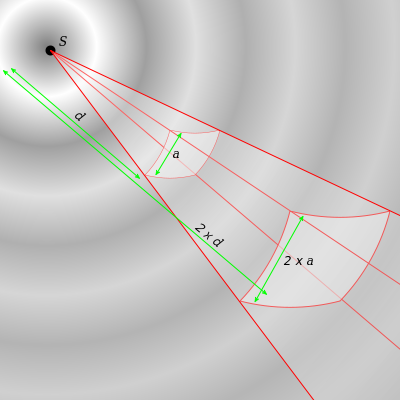
\includegraphics[width=\textwidth]{flux}
		\caption{Representation of the distribution of the energy flow in the propagation of a spherical wave.}
		\label{flux}
	\end{subfigure}
	\begin{subfigure}{0.6\textwidth}
		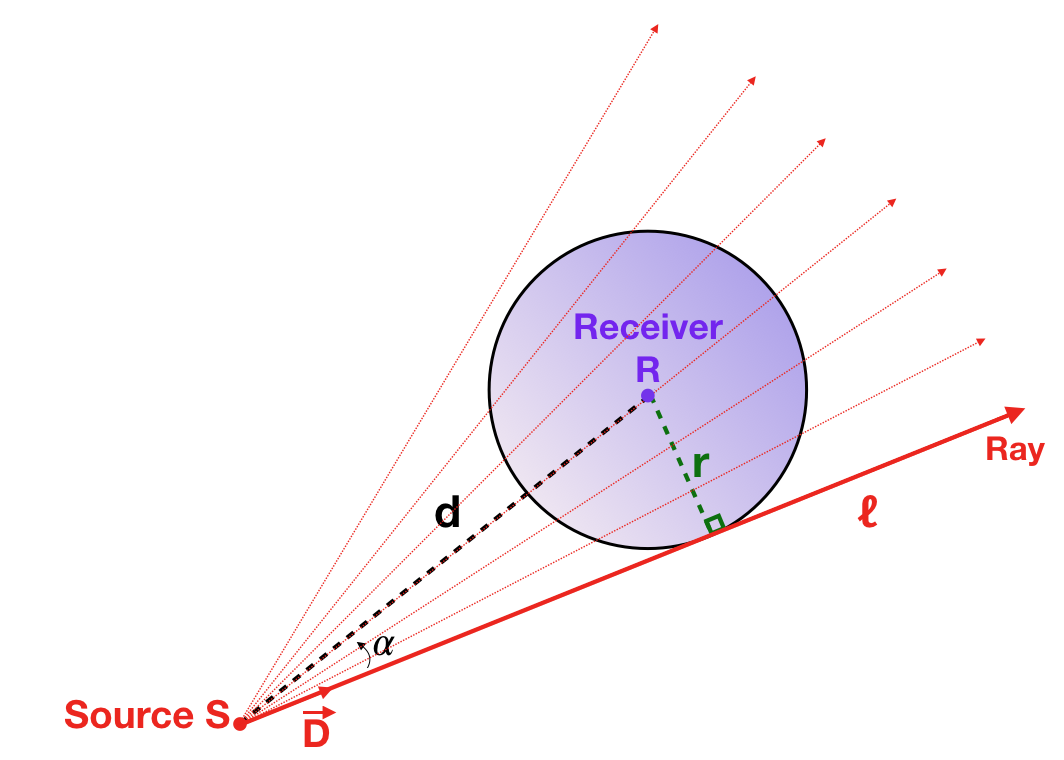
\includegraphics[width=\textwidth]{rays}
		\caption{Representation of rays mesure by a receiver.}
		\label{rays}
	\end{subfigure}	
	\caption{Acoustic emission from a point source.}
\end{figure}

We understand that the intensity decreases as the square of the distance and that a portion of energy considered will therefore be carried by a solid angle (see fig. \ref{flux}). Thus, at a distance $d$ the same amount of energy is distributed over an area of $a^2$ as at a distance of $2d$ over an area of $(2a)^2$. The energy is distributed over an area proportional to the square of the distance. On a portion of $S(t)$ the energy is carried by a solid angle $\Omega_{S}$ such as :
%
\begin{equation} \label{eq_energie}
E_{S}(t) = E_0 \int_{S(t)}  \frac{1}{4\pi  d(t)^2} dS = \frac{E_0}{4\pi}  \Omega_{S}.
\end{equation}
%
This reflects the fact that the energy of a solid angle is constant over time and corresponds to a portion of the initial energy $E_0$. We can then consider the total energy as the sum of energies carried by solid angles such as : 

\begin{equation}
E(t) = \sum_{i=1}^N E_i(t) = \frac{E_0}{4\pi}  \sum_{i=1}^N \Omega_i  \qquad \forall t > 0,
\end{equation}
with  $\Omega_i$ the elementary solid angle : $ \sum_{i=1}^N \Omega_i = 4\pi$. \\

We have chosen to represent each solid angle $ \Omega_i$ by a vector $u_i$, which we will call "ray", and which gives the direction of propagation of the energy $E_i(t)$ over time. Thus, to measure the acoustic energy E(x; t) at a given point in space, we can consider a measuring sphere S(x; r), centred at x and radius r. We can then add the contributions of the n rays that intersect this sphere to calculate the acoustic energy at point x :

\begin{equation}
E(t) = \frac{E_0}{4\pi}\Omega_{S(x,r)} = \frac{E_0}{4\pi}  \sum_{i=1}^n \Omega_i,
\end{equation}

However, to be able to statistically assimilate a set of n rays to a continuous portion of a sphere, it must be ensured that n is large. We use omnidirectional sources, so we can write:
\begin{equation}
	\Omega_i = \frac{4\pi}{N}.
\end{equation}
%
and, by using the formula of a solid angle in a cône, if we consider d, the distance between the source and the receiver sphère S(x; r), we obtain :
\begin{equation}
	\Omega_{S(x,r)} = 4\pi \frac{n}{N} = 2\pi \left(1- \frac{\sqrt{d^2-r^2}}{d}\right).
\end{equation}
%
By fixing n (a number minimum of rays to be caught) and r (the receiver radius) we can get the maximum length of the rays before the measurement become statistically inaccurate :

\begin{equation}
	d_{max} =  \frac{N.r}{2n\sqrt{\frac{N}{n}-1}}.
\end{equation}
%
For large rooms, the total number of rays will be significant (typically N >$10^6$ and n >100) to preserve an accurate measure.

%Example for bibliography citations cite\cite{Taylor1937}, cites\cite{Knupp1999,Kamm2000}

%\begin{figure}[t]
%\centerline{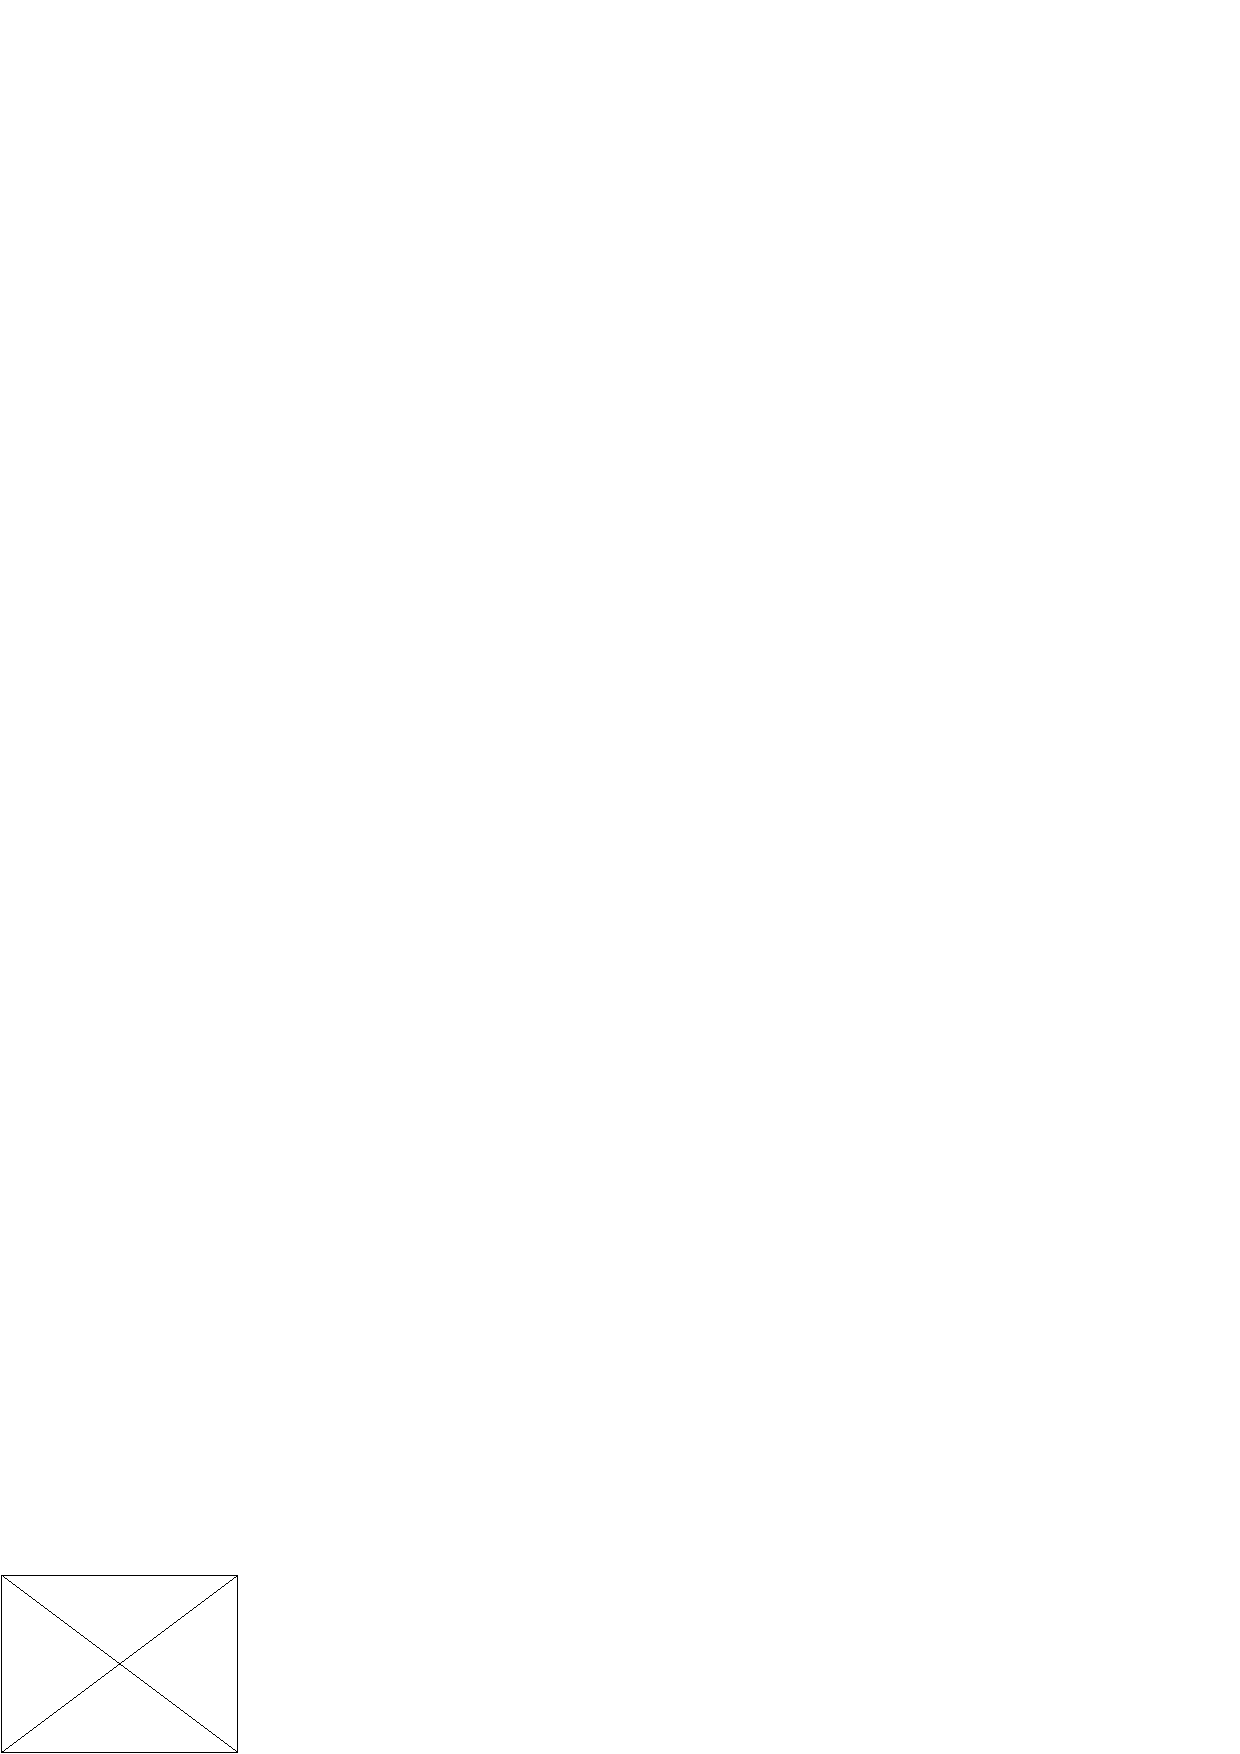
\includegraphics[width=342pt,height=9pc,draft]{empty}}
%\caption{This is the sample figure caption.\label{fig1}}
%\end{figure}



%\subsection{Example for second level head}


\section{Hybride Ray-Tracing / Image-Source methode}\label{sec3}

The method developed aims to propagate rays from a point source. A ray is define with the following equation (see fig .\ref{rays}) :
\begin{equation}
\overrightarrow{R}(d) = O + \overrightarrow{D}.d,
\end{equation}
where :
\begin{itemize}
\item $O$ is the origine of the ray,
\item $\overrightarrow{D}$ is the unitary orientation vecteur.
\end{itemize}

To generate $N$ uniform rays, we use a Fibonacci sphere. We note $\Gamma$ the golden ratio such as :
\begin{equation}
\Gamma = \frac{1 + \sqrt{5}}{2}. \\
\end{equation}
%
The spherical coordinates are given by :
\begin{equation}
  \left \{
   \begin{array}{r c l}
\theta &=& \frac{2 \pi \times n}{\Gamma}  \pmod{2\pi},  \\
\phi &=& \arcsin{\left(\frac{2n}{N-1}-1\right)}, 
   \end{array}
   \right .
\end{equation}
%
with : 
\begin{itemize}
\item $N$ : the total number of rays,
\item $n \in[0, 1, 2, \ ... \ ,N-1]$ : the index of the ray.
\end{itemize}
%
Once convert into cartesian coordinates and normalized we can test the intersection with the triangles of the mesh. If a ray intersect a triangle, we can find a point T such as :

\begin{equation} \label{eq_2moller}
T(u,v) = (1-u-v)V_0 + uV_1 + vV_2 = O + D.d,% \ \ \ \footnotemark
\end{equation}
%\citefnt[eq. 2]{moller}
%
with $(u,v)$ the barycentric coordinates such as :
\begin{equation}
   \left \{
   \begin{array}{r c l}
u & \geqslant & -\epsilon,  \\
v & \geqslant & -\epsilon,  \\
(u+v) & \leqslant & 1+\epsilon,
   \end{array}
   \right .
\end{equation}
where $\epsilon = 10^{-5}$ to avoid rounding errors due to machine precision. $d$ is the distance between the point of origin of the ray and the point of intersection. According to Cramer's rule, we can rearrange this equation into the form : :
%
\begin{equation}
	\begin{bmatrix}
 	  -D, & V_1-V_0, & V_2-V_0
	\end{bmatrix}
	\begin{bmatrix}
 	 d \\
	 u \\
	 v
	\end{bmatrix}
	= O-V_0.
	%\ \ \ \footnotemark
\end{equation}
%\citefnt[eq. 4]{moller}
%
Then we get :
\begin{equation}
	\begin{bmatrix}
 	 d \\
	 u \\
	 v
	\end{bmatrix}
	=
	\frac{1}{
	\begin{vmatrix}
 	  -D, & E_1, & E_2
	\end{vmatrix}
	}
	\begin{bmatrix}
 	 	\begin{vmatrix}
 		  T, & E_1, & E_2
		\end{vmatrix} \\
 	 	\begin{vmatrix}
 		  -D, & T, & E_2
		\end{vmatrix} \\
 	 	\begin{vmatrix}
 		  -D, & E_1, & T
		\end{vmatrix}
	\end{bmatrix}	.
	%\footnotemark
\end{equation}
%\citefnt[eq. 5]{moller}
%
with : 
\begin{equation}
   \left \{
   \begin{array}{r c l}
E_1 &=&  V_1-V_0,  \\
E_2 &=&  V_2-V_0,  \\
T &=& O - V_0.
   \end{array}
   \right .
\end{equation}
%
This can be written : 
%
\begin{equation}
	\begin{bmatrix}
 	 d \\
	 u \\
	 v
	\end{bmatrix}
	=
	\frac{1}{
 	  (D \times E_2).E_1
	}
	\begin{bmatrix}
 		  (T \times E_1).E_2
 \\ 
 		  (D \times E_2).T
 \\
 		  (T \times E_1).D
	\end{bmatrix}	.
	%\footnotemark
\end{equation}
%\citefnt[eq. 6]{moller}

The rays can then be reflected on the face as on a mirror to find the new orientation vector :
\begin{equation}
\overrightarrow{r} - \overrightarrow{i} = 2 \times (-\overrightarrow{i}.\overrightarrow{n})\overrightarrow{n}.
\end{equation}
with : 
\begin{itemize}
\item $\overrightarrow{r}$ : the reflected ray,
\item $\overrightarrow{i}$ : the incident ray,
\item $\overrightarrow{n}$ : the normal of the face.
\end{itemize}

\begin{figure}
\centering
	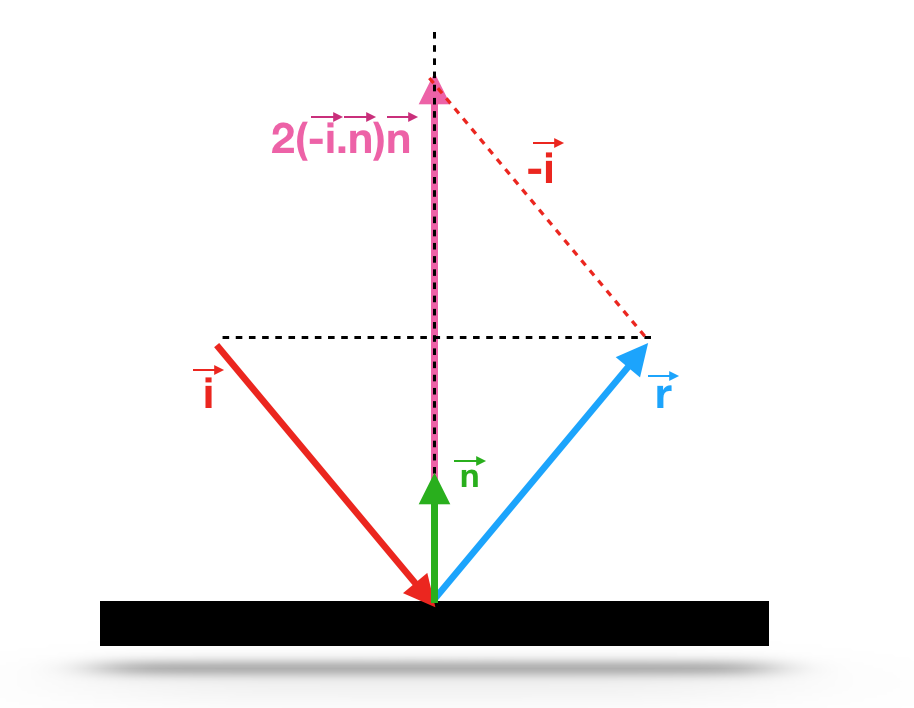
\includegraphics[width=0.4\linewidth]{rayRefl}
	\caption{Calculation of a reflected ray from an incident ray and a normal ray}
	\label{rayRefl}
\end{figure}

Once we know the elements met be each ray we can update their energies. Each triangle carries an an absorption coefficient $\alpha_i$ for every octave band (from 62,5Hz to 8kHz). Moreover, we take into account the atmospheric attenuation. The energy of a ray is :
\begin{equation}
E_{i} =  \frac{E_0}{N} \times \prod_{j=0}^{k}{(1-\alpha_{i,j})} \times e^{-m_i . d_{tot}},
\end{equation}
with : 
\begin{itemize}
\item $E_{i}$ : the energy carried by the ray on the i-th frequency band,
\item $E_{0}$ : the total energy,
\item $k$ : the total number of faces encountered by the rays during its propagation,
\item $j$ : the index of the face encountered par the ray,
\item $m_i$ : the air absorption coefficient in the i-th frequency band (according to the norm ISO-9613),
\item $ d_{tot}$ : the total length of the ray.
\end{itemize}

At each ray bounce, we check if the rays intersect the receiver-sphere. This test includes the following steps :
First we check if the origine point $O$ of the ray is include in the R-center and r-radius receiver :
\begin{equation}
||\overrightarrow{OR}|| \leqslant r,
\end{equation}
%
If not, we check the direction of the ray :
\begin{equation}
\cos{\alpha} \geqslant 0,
\end{equation}
with $\alpha$ the angle between the ray $\overrightarrow{D}$ and $\overrightarrow{OR}$. Then we check if the ray is long enough to reach the receiver :

\begin{equation}
||\overrightarrow{OR}|| \leqslant d,
\end{equation}
%
To finish, we check if the ray intersect the receiver-sphere :

\begin{align}
\sin{\alpha} \times ||\overrightarrow{OR}||  \leqslant r 
\quad \Rightarrow \quad
\alpha  \leqslant \arcsin{\frac{r}{||\overrightarrow{OR}||}}
\end{align}

If the ray deos indeed intersect the receiver an image-source is generated. This is the image of the sound source relative to all the walls encountered by the ray. The image-source SI is located in space by back-propagation of the ray from its last origin point O :

\begin{equation}
\overrightarrow{SI} = O - D.d_{tot},
\end{equation}
where 
\begin{itemize}
\item $D$ is the last orientation vector of the ray,
\item $d_{tot}$ is the total distance travelled by the ray from the original source to the point O .
\end{itemize}

\begin{figure}
\centering
	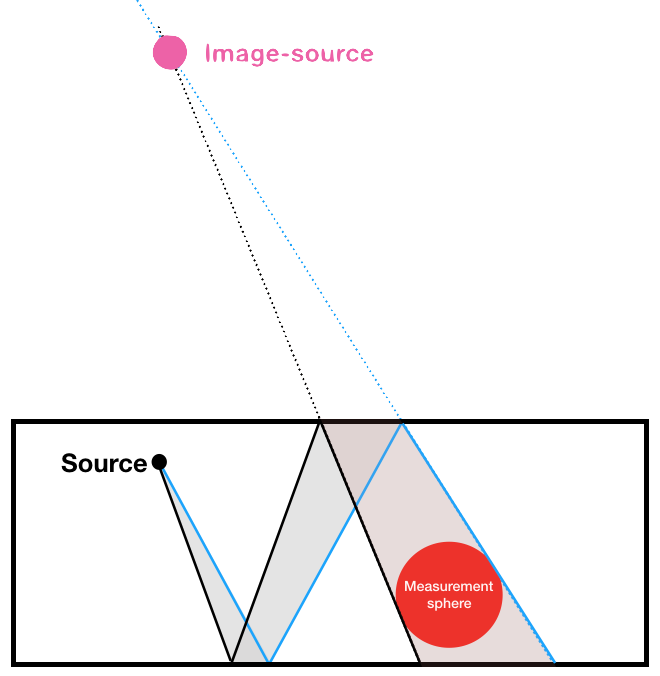
\includegraphics[width=0.3\linewidth]{schema_SI}
	\caption{Sketch of the creation of an image-source by successive reflections of a ray on the walls of a room}
	\label{schema_SI}
\end{figure}

\section{Algorithm's optimisation}\label{sec4}

\section{Validation}\label{sec5}

\section{Developed softwares }\label{sec6}

\section{Application to the antic theatre of Orange}\label{sec7}


\section{Conclusions}

\section*{Acknowledgments}


\subsection*{Author contributions}

This is an author contribution text. This is an author contribution text. This is an author contribution text. This is an author contribution text. This is an author contribution text. 

\subsection*{Financial disclosure}

None reported.

\subsection*{Conflict of interest}

The authors declare no potential conflict of interests.


\section*{Supporting information}

The following supporting information is available as part of the online article:

\noindent
\textbf{Figure S1.}
{500{\uns}hPa geopotential anomalies for GC2C calculated against the ERA Interim reanalysis. The period is 1989--2008.}

\noindent
\textbf{Figure S2.}
{The SST anomalies for GC2C calculated against the observations (OIsst).}


\appendix

\section{Section title of first appendix\label{app1}}

Use \verb+\begin{verbatim}...\end{verbatim}+ for program codes without math. Use \verb+\begin{alltt}...\end{alltt}+ for program codes with math. Based on the text provided inside the optional argument of \verb+\begin{code}[Psecode|Listing|Box|Code|+\hfill\break \verb+Specification|Procedure|Sourcecode|Program]...+ \verb+\end{code}+ tag corresponding boxed like floats are generated. Also note that \verb+\begin{code}[Code|Listing]...+ \verb+\end{code}+ tag with either Code or Listing text as optional argument text are set with computer modern typewriter font.  All other code environments are set with normal text font. Refer below example:

\begin{lstlisting}[caption={Descriptive Caption Text},label=DescriptiveLabel]
for i:=maxint to 0 do
begin
{ do nothing }
end;
Write('Case insensitive ');
WritE('Pascal keywords.');
\end{lstlisting}



\subsection{Subsection title of first appendix\label{app1.1a}}

\noindent\textbf{Unnumbered figure}


\begin{center}
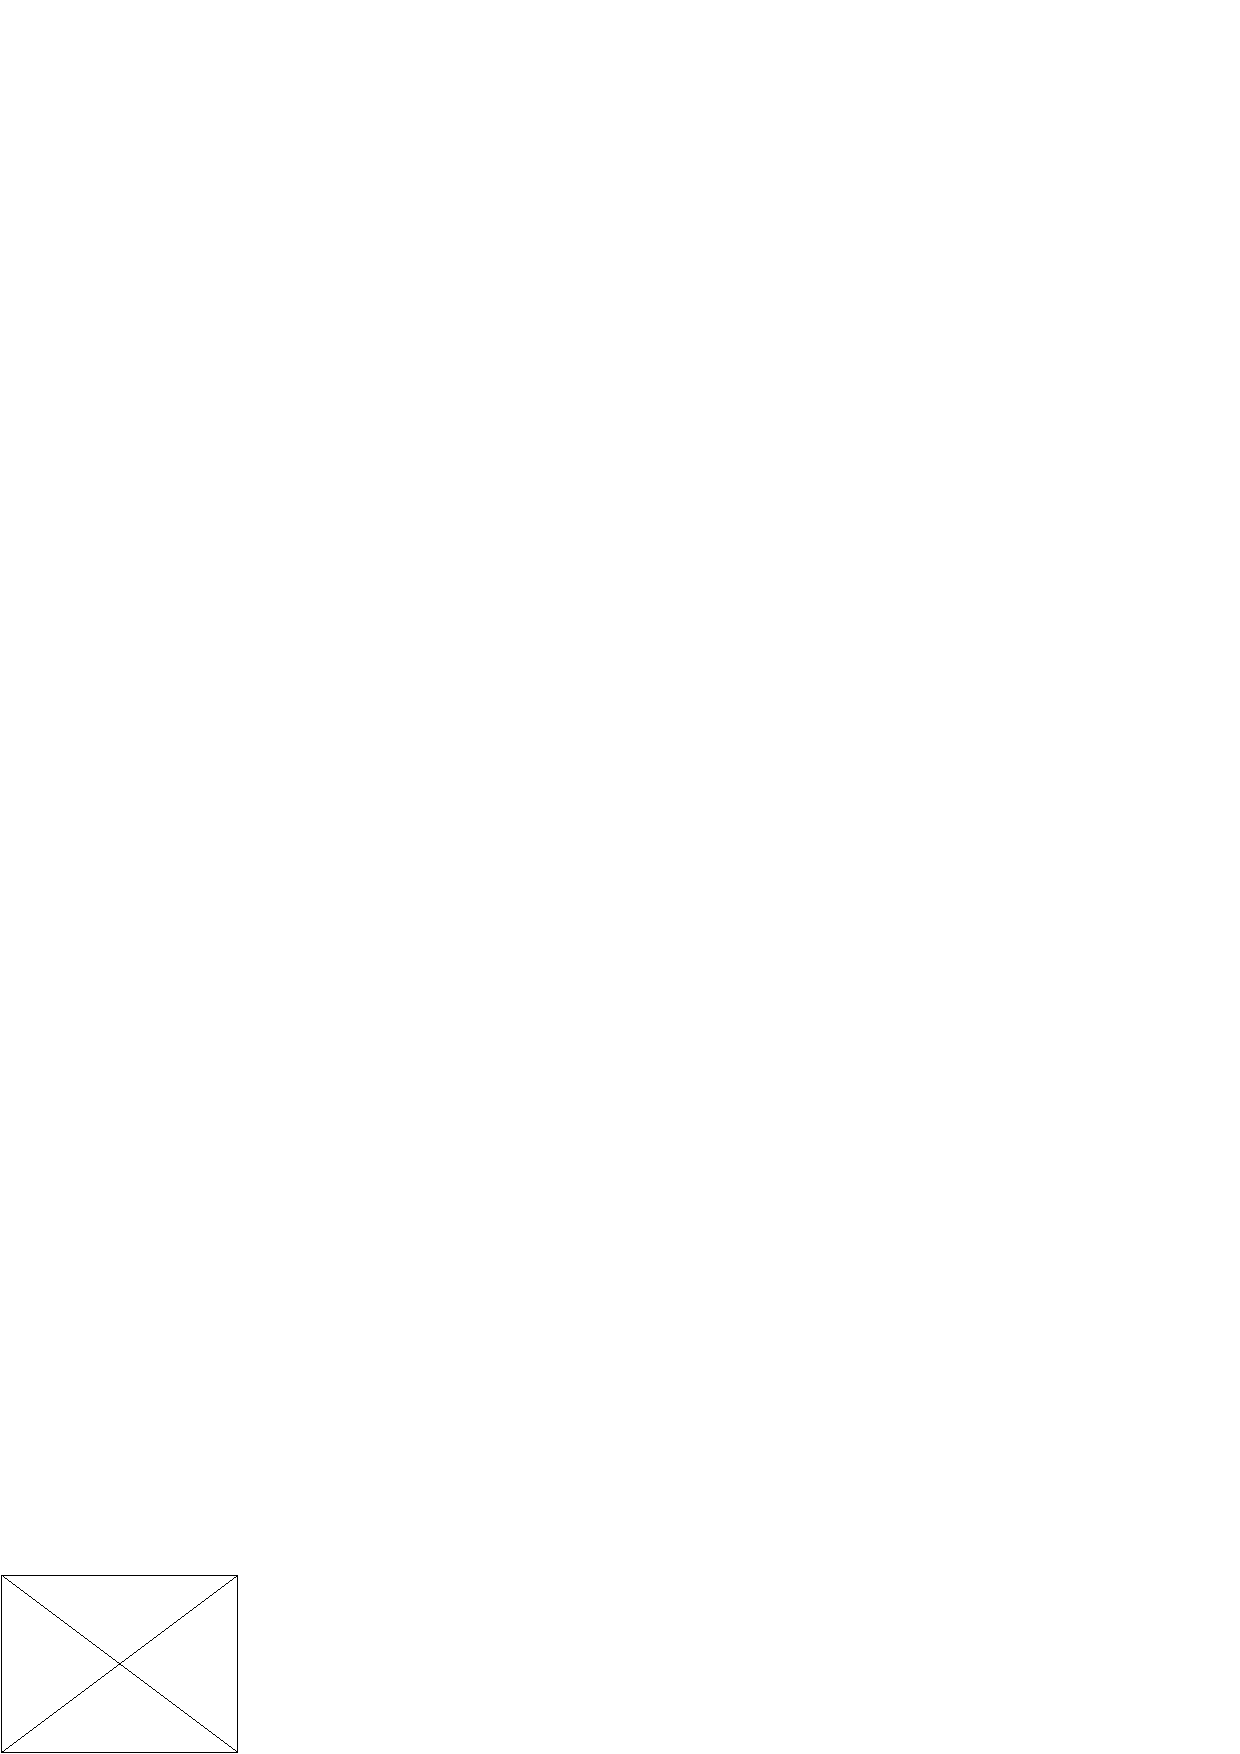
\includegraphics[width=7pc,height=8pc,draft]{empty}
\end{center}


%== Figure 4 ==
%% Example for figure inside appendix
\begin{figure}[t]
\centerline{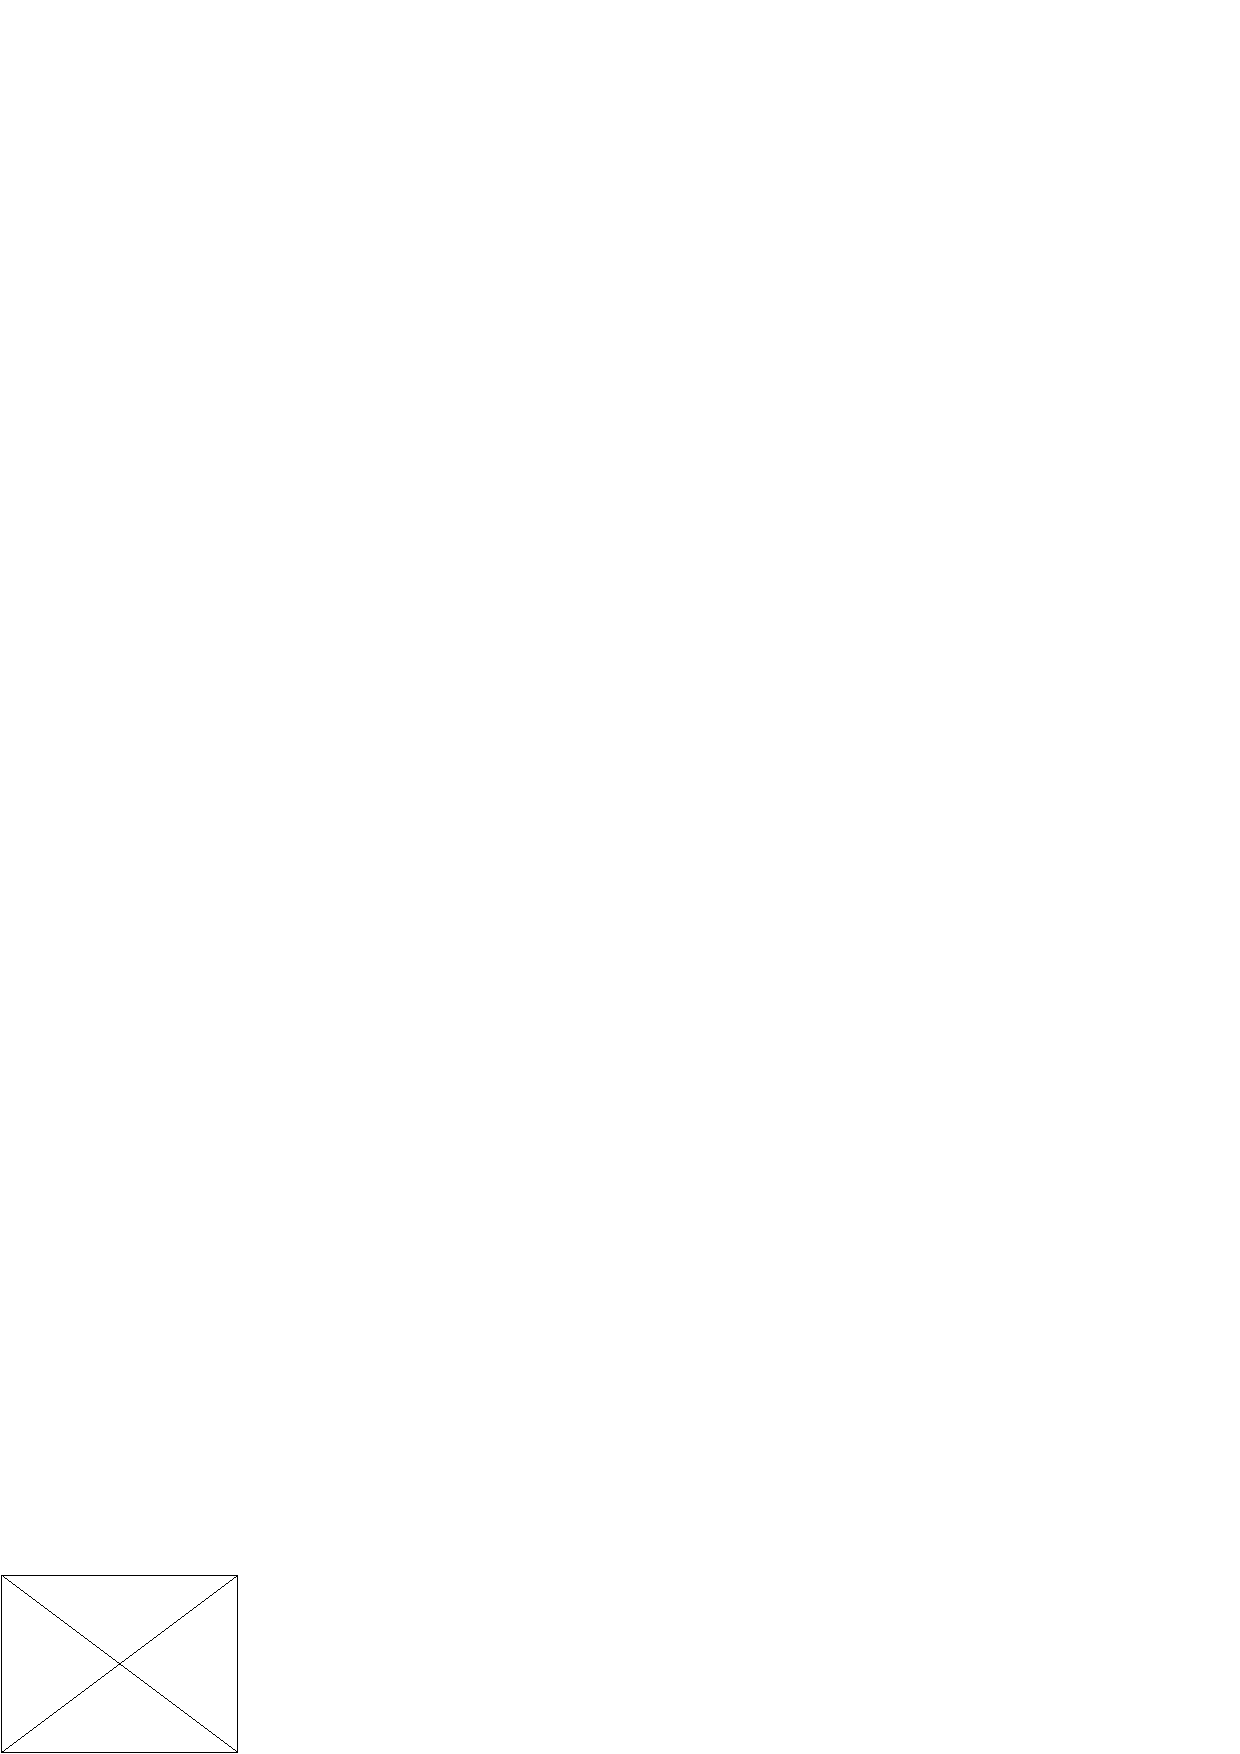
\includegraphics[height=10pc,width=78mm,draft]{empty}}
\caption{This is an example for appendix figure.\label{fig5}}
\end{figure}


\nocite{*}% Show all bib entries - both cited and uncited; comment this line to view only cited bib entries;
\bibliography{Biblio}%

\clearpage

\section*{Author Biography}

\begin{biography}{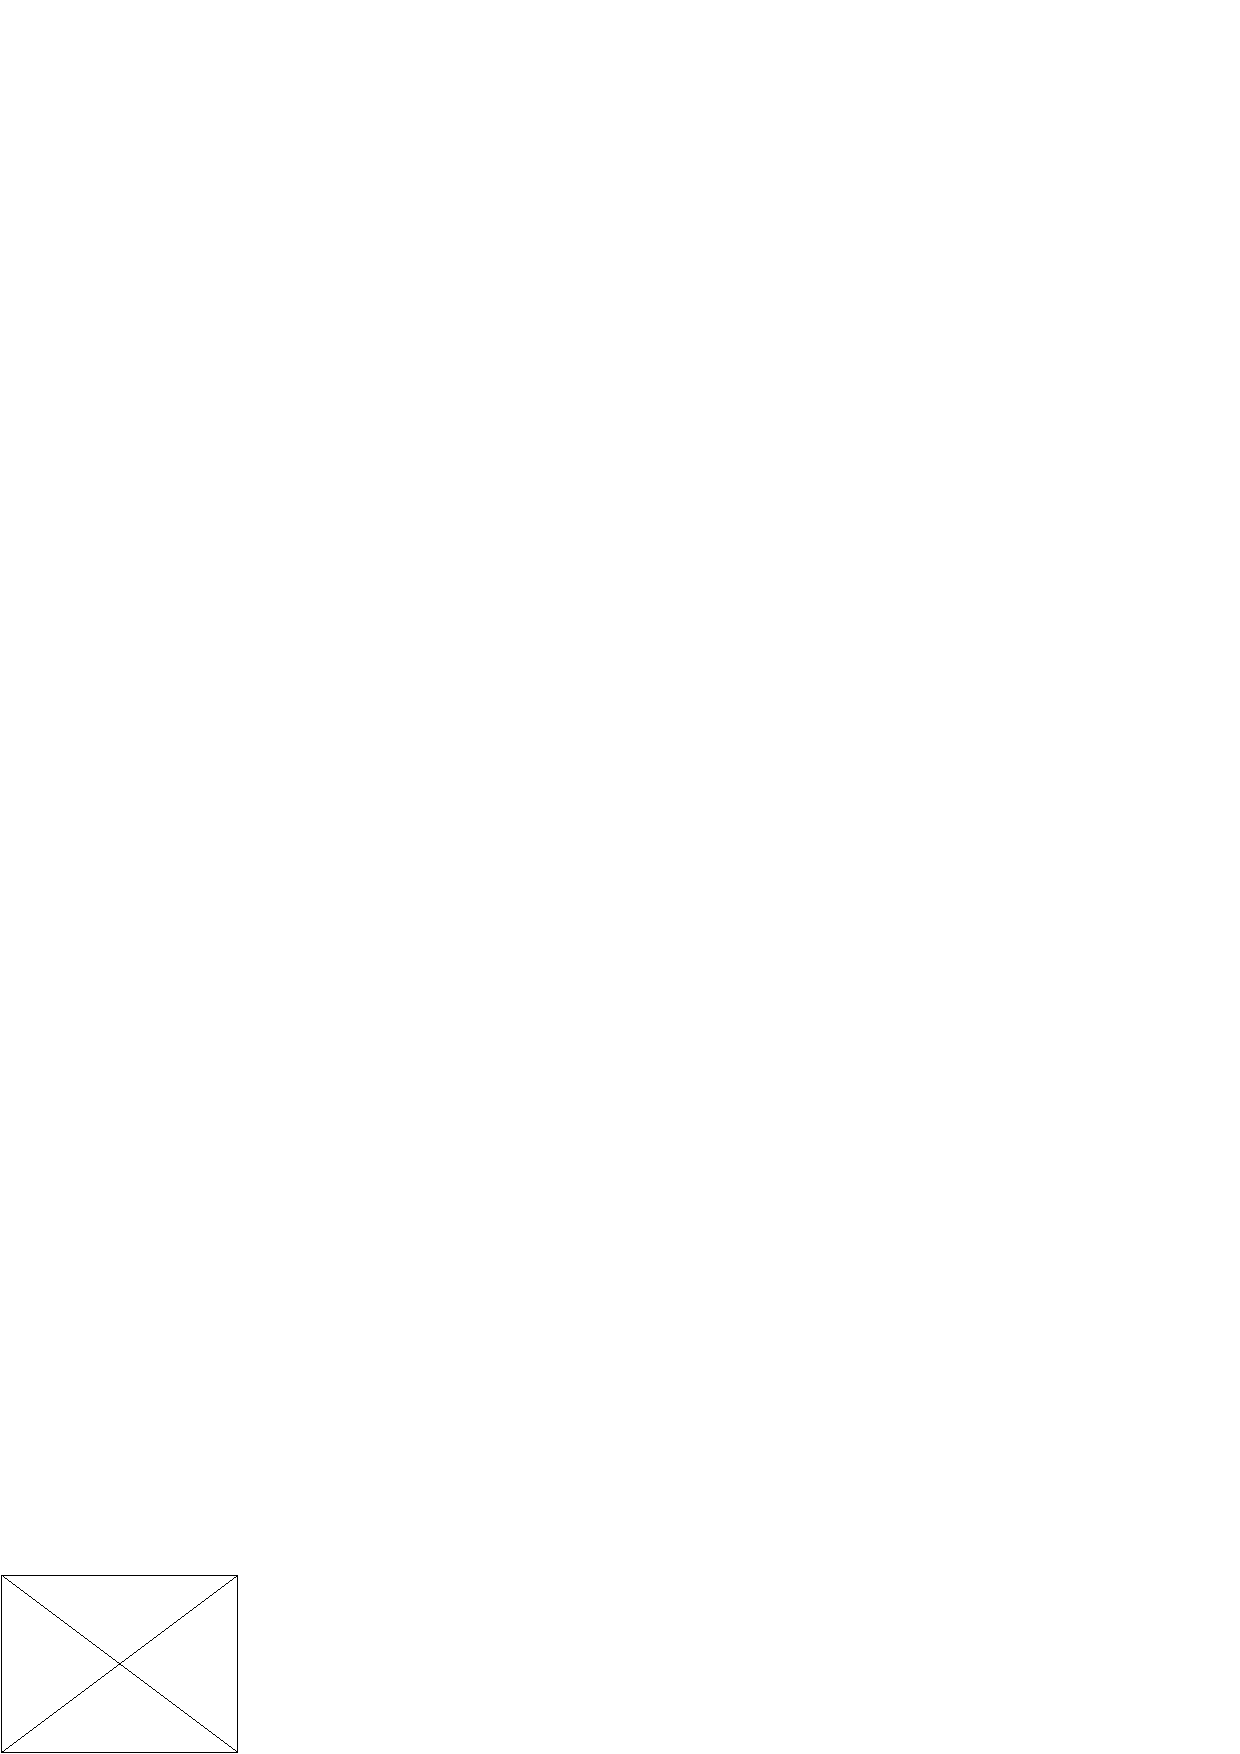
\includegraphics[width=66pt,height=86pt,draft]{empty}}{\textbf{Author Name.} This is sample author biography text this is sample author biography text this is sample author biography text this is sample author biography text this is sample author biography text this is sample author biography text this is sample author biography text this is sample author biography text this is sample author biography text this is sample author biography text this is sample author biography text this is sample author biography text this is sample author biography text this is sample author biography text this is sample author biography text this is sample author biography text this is sample author biography text this is sample author biography text this is sample author biography text this is sample author biography text this is sample author biography text.}
\end{biography}

\end{document}
